\section{Training of the kinematic BDT discriminators}
\label{app:BDTtraining}

We train two BDTs aiming at separating the signal from the \ttV\, \ttbar\ backgrounds respectively, using the input variables described in Section~\ref{sec:extraction}.

All trainings are performed on samples that are not used anywhere else in the signal extraction (Powheg \ttH\, leading order \ttV\, and pure \ttbar\ MC).

\subsection*{2lss event category, \ttbar\ training}
\begin{figure}[htb]
 \centering
 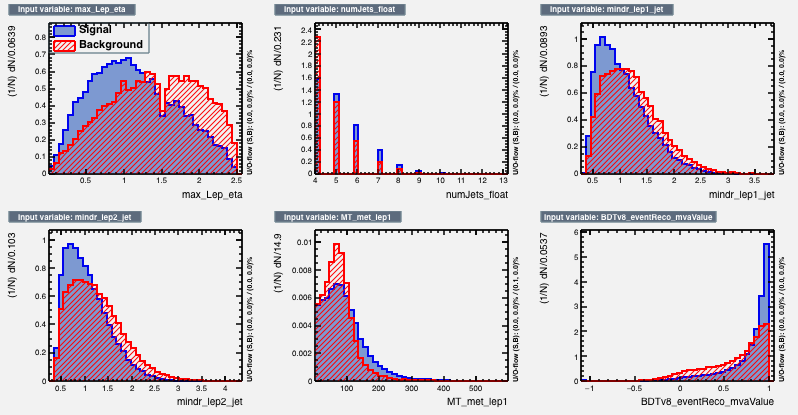
\includegraphics[width=\textwidth]{plots_extraction/training/train_2lss_ttbar_bdtv8_value/variables_id_c1}\\
 \includegraphics[width=\textwidth]{plots_extraction/training/train_2lss_ttbar_bdtv8_value/variables_id_c2}\\
\end{figure}
\begin{figure}[htb]
 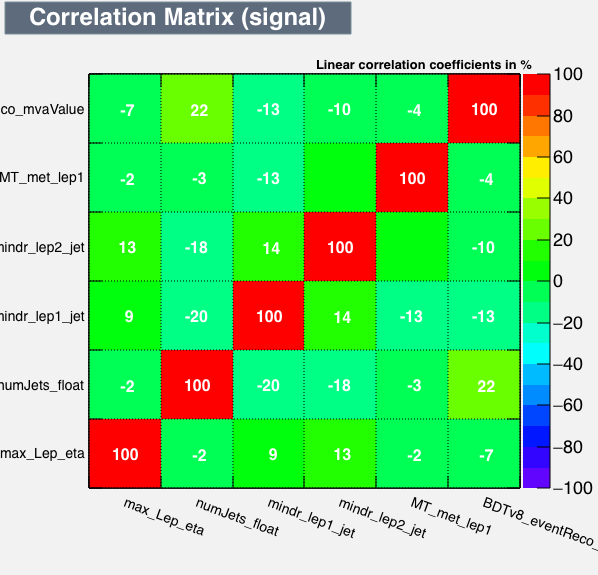
\includegraphics[width=0.32\textwidth]{plots_extraction/training/train_2lss_ttbar_bdtv8_value/CorrelationMatrixS}
 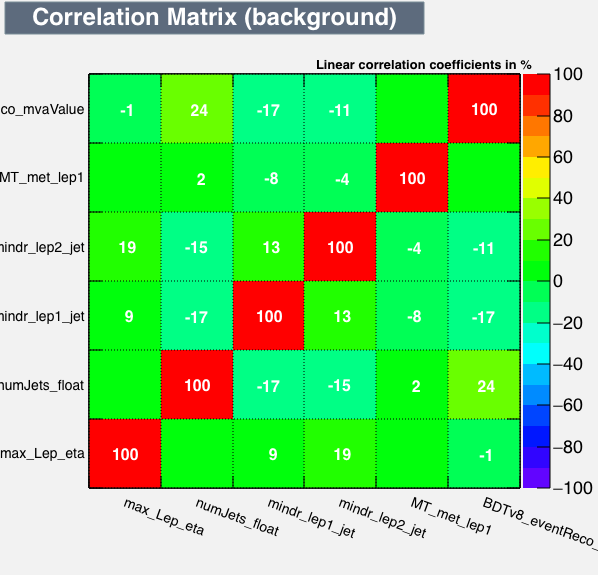
\includegraphics[width=0.32\textwidth]{plots_extraction/training/train_2lss_ttbar_bdtv8_value/CorrelationMatrixB}
 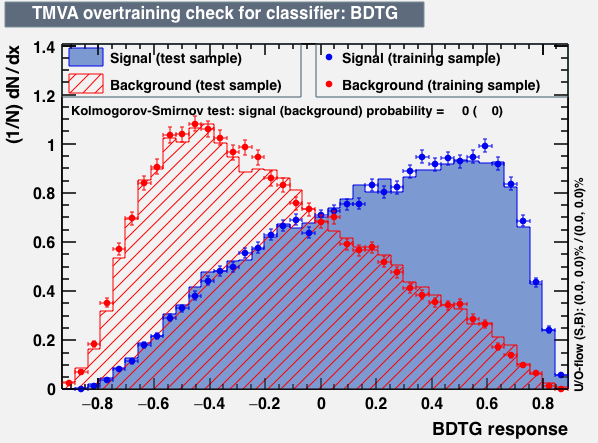
\includegraphics[width=0.32\textwidth]{plots_extraction/training/train_2lss_ttbar_bdtv8_value/overtrain_BDTG.png}
\end{figure}

\clearpage

\subsection*{2lss event category, \ttV\ training}
\begin{figure}[htb]
 \centering
 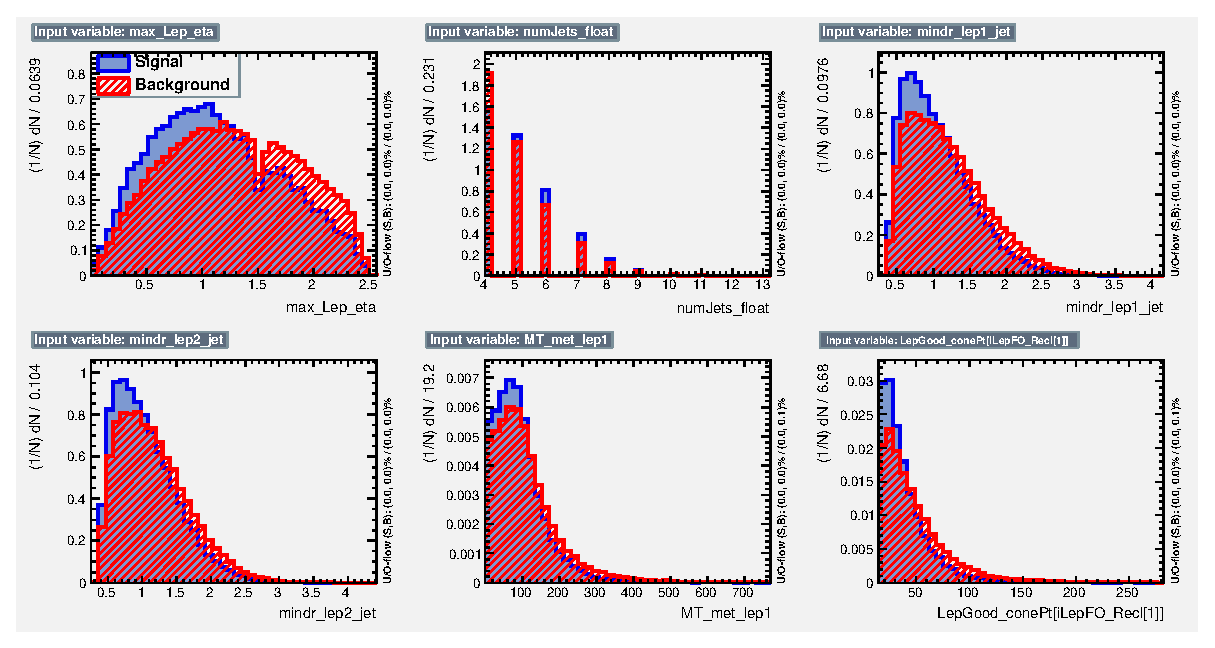
\includegraphics[width=\textwidth]{plots_extraction/training/train_2lss_ttv_hj_value/variables_id_c1}\\
 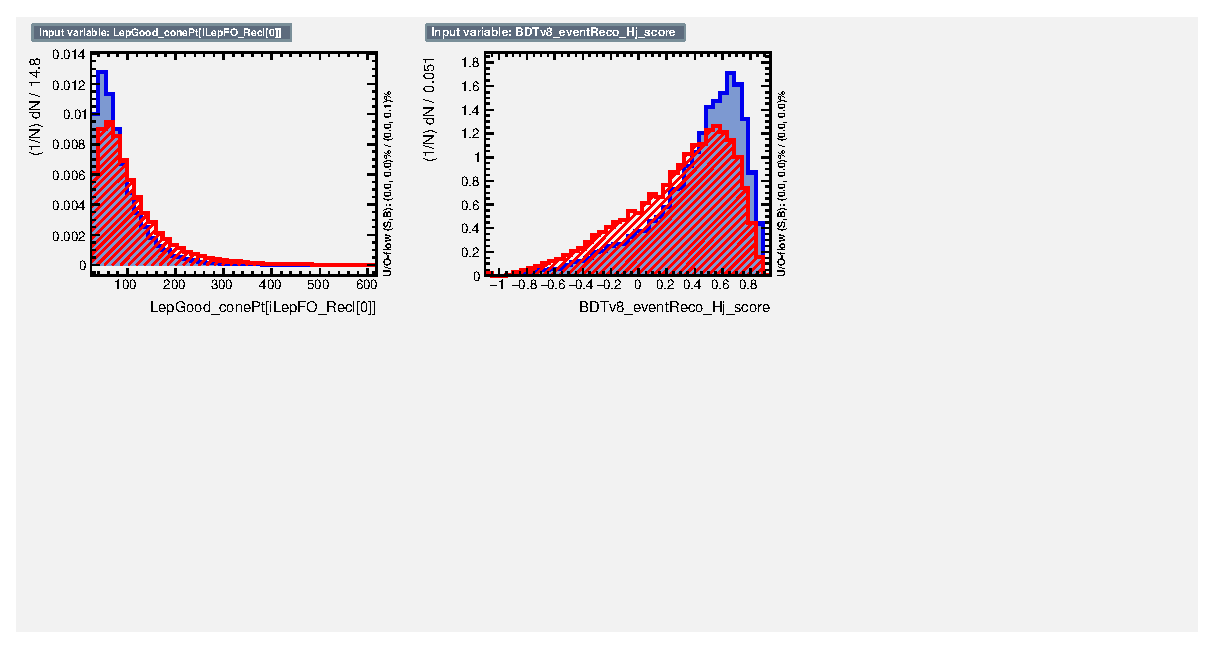
\includegraphics[width=\textwidth]{plots_extraction/training/train_2lss_ttv_hj_value/variables_id_c2}\\
\end{figure}
\begin{figure}[htb]
 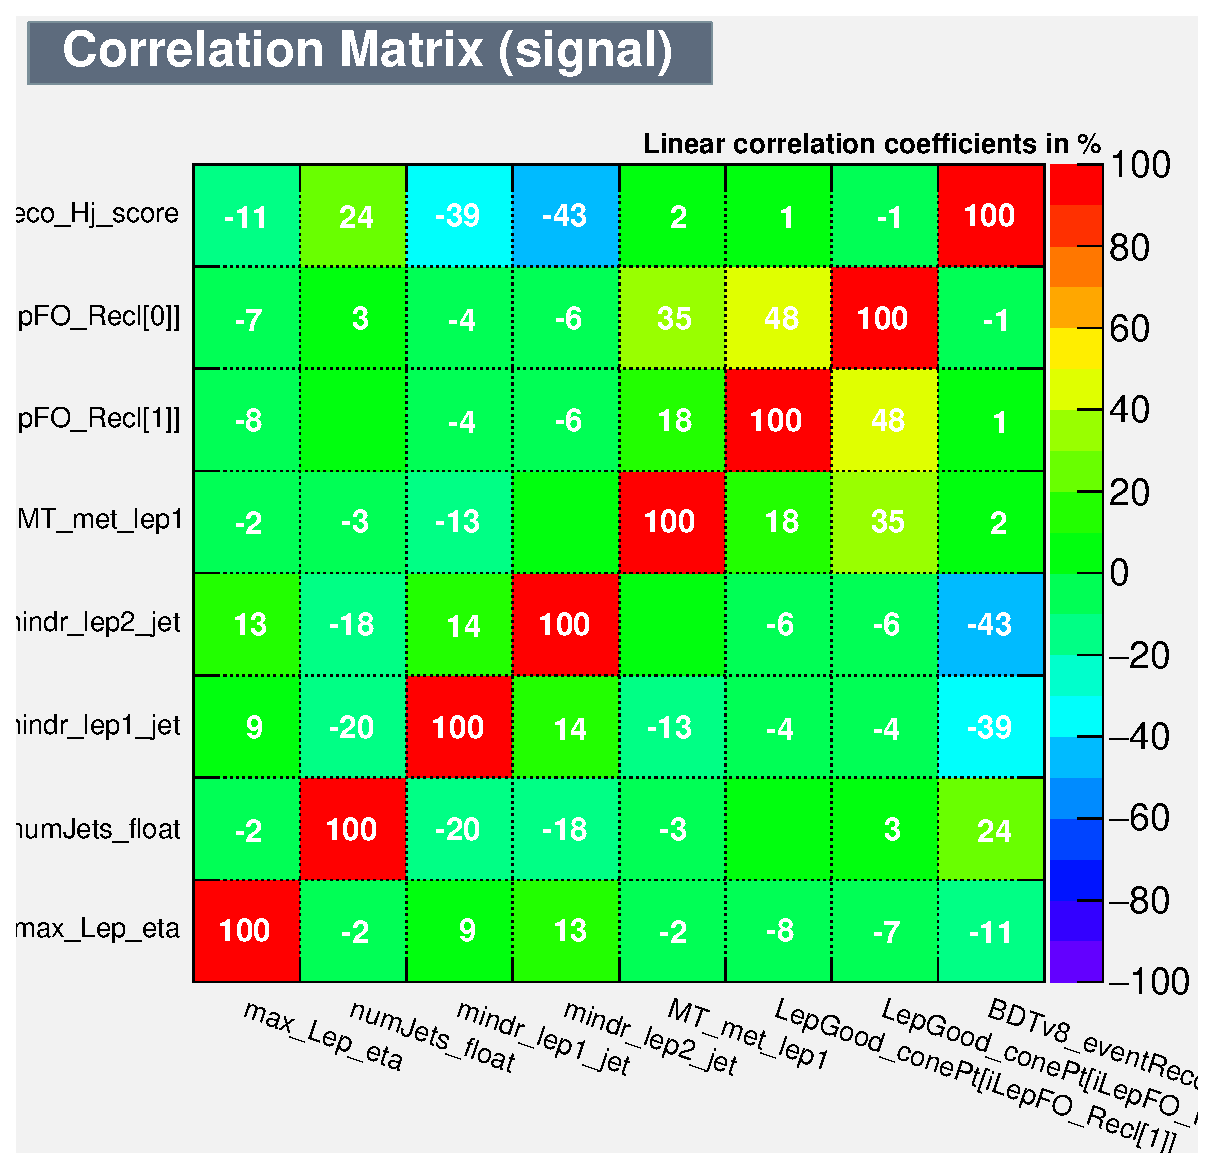
\includegraphics[width=0.32\textwidth]{plots_extraction/training/train_2lss_ttv_hj_value/CorrelationMatrixS}
 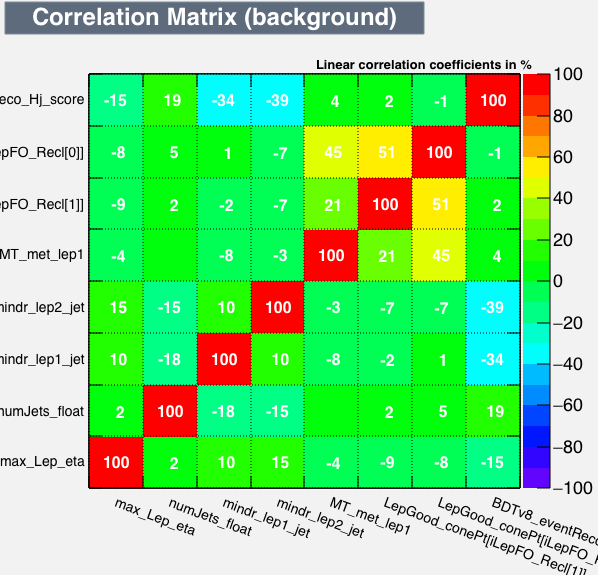
\includegraphics[width=0.32\textwidth]{plots_extraction/training/train_2lss_ttv_hj_value/CorrelationMatrixB}
 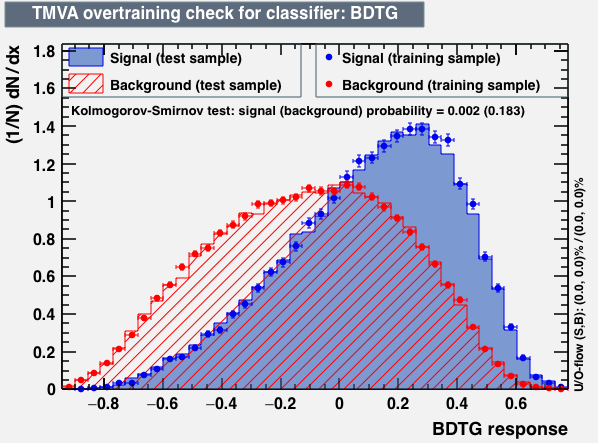
\includegraphics[width=0.32\textwidth]{plots_extraction/training/train_2lss_ttv_hj_value/overtrain_BDTG.png}
\end{figure}

\clearpage

\subsection*{3l event category, \ttbar\ training}
\begin{figure}[htb]
 \centering
 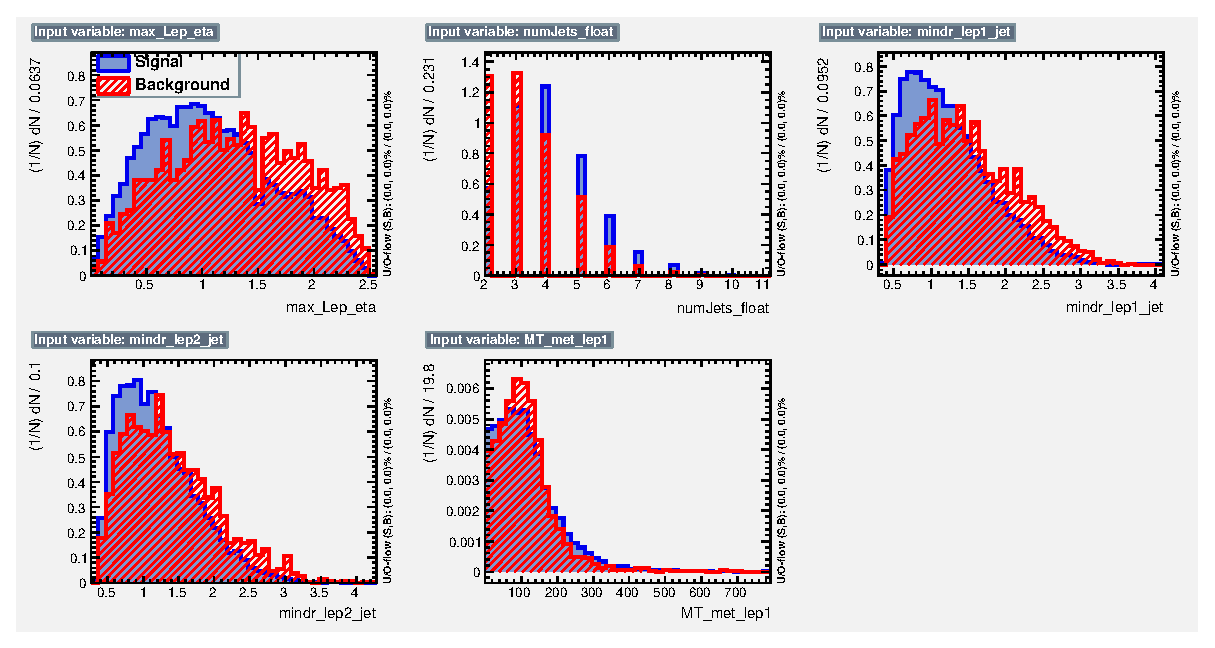
\includegraphics[width=\textwidth]{plots_extraction/training/train_3l_ttbar/variables_id_c1}\\
\end{figure}
\begin{figure}[htb]
 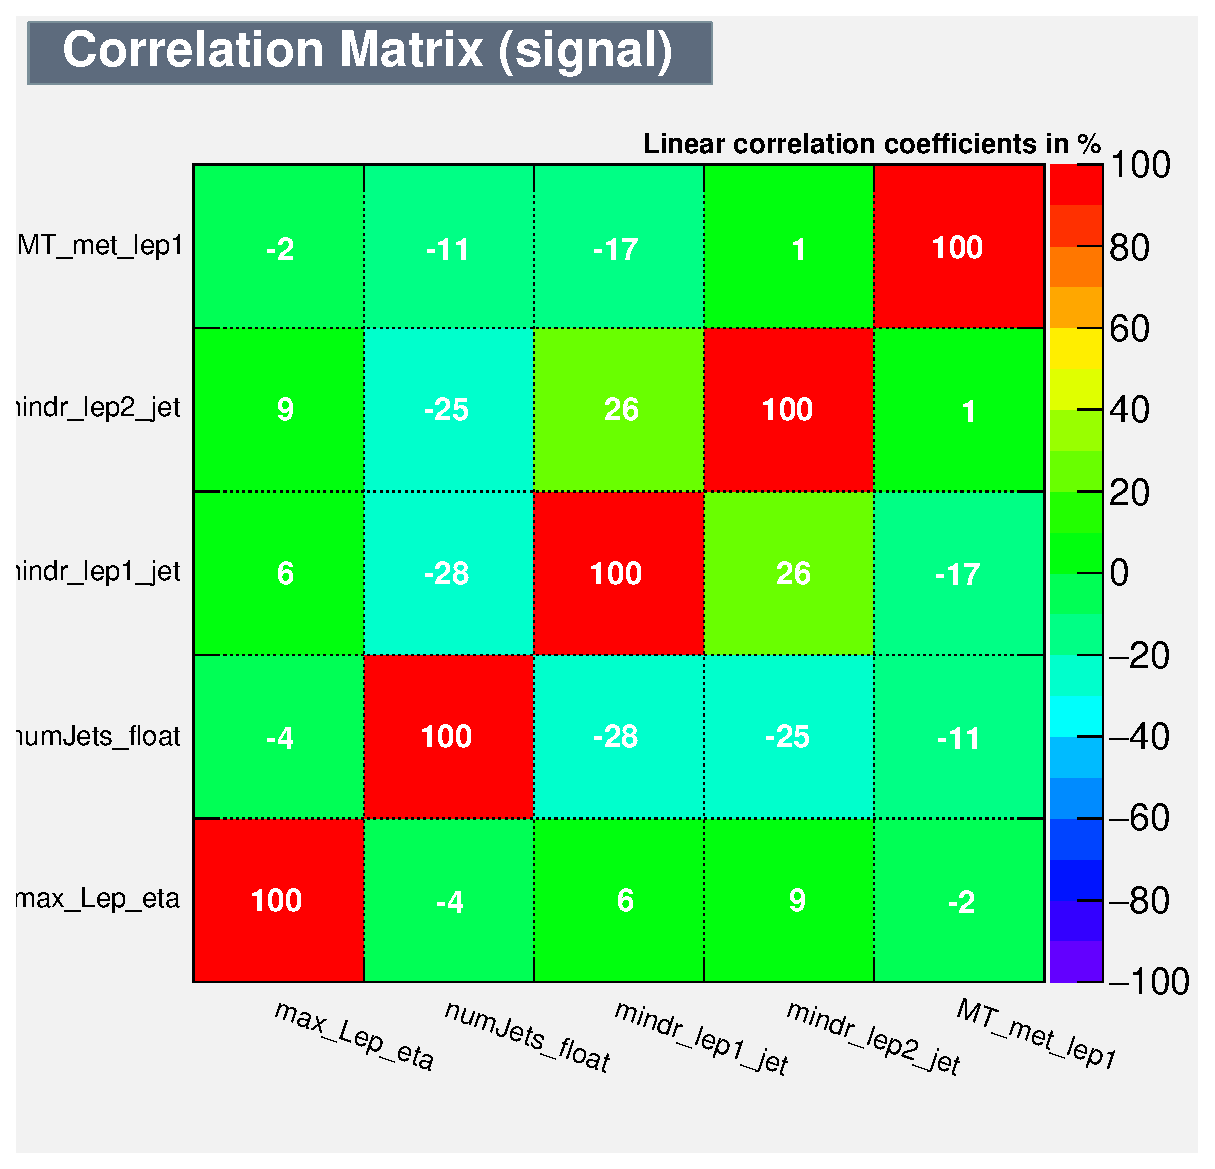
\includegraphics[width=0.32\textwidth]{plots_extraction/training/train_3l_ttbar/CorrelationMatrixS}
 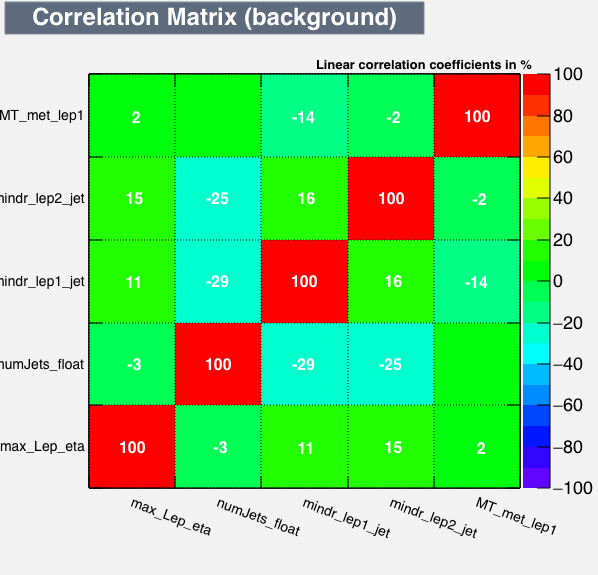
\includegraphics[width=0.32\textwidth]{plots_extraction/training/train_3l_ttbar/CorrelationMatrixB}
 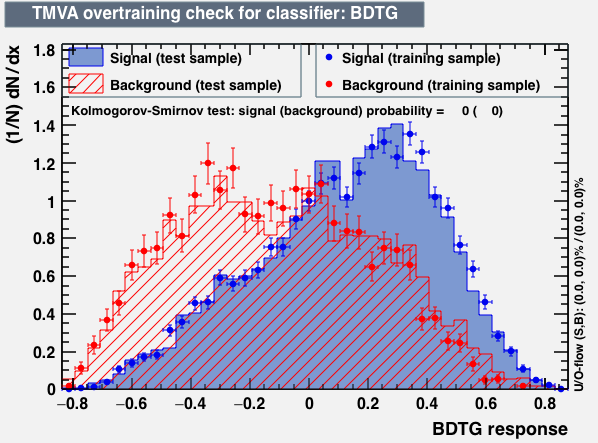
\includegraphics[width=0.32\textwidth]{plots_extraction/training/train_3l_ttbar/overtrain_BDTG.png}
\end{figure}

\clearpage

\subsection*{3l event category, \ttV\ training}
\begin{figure}[htb]
 \centering
 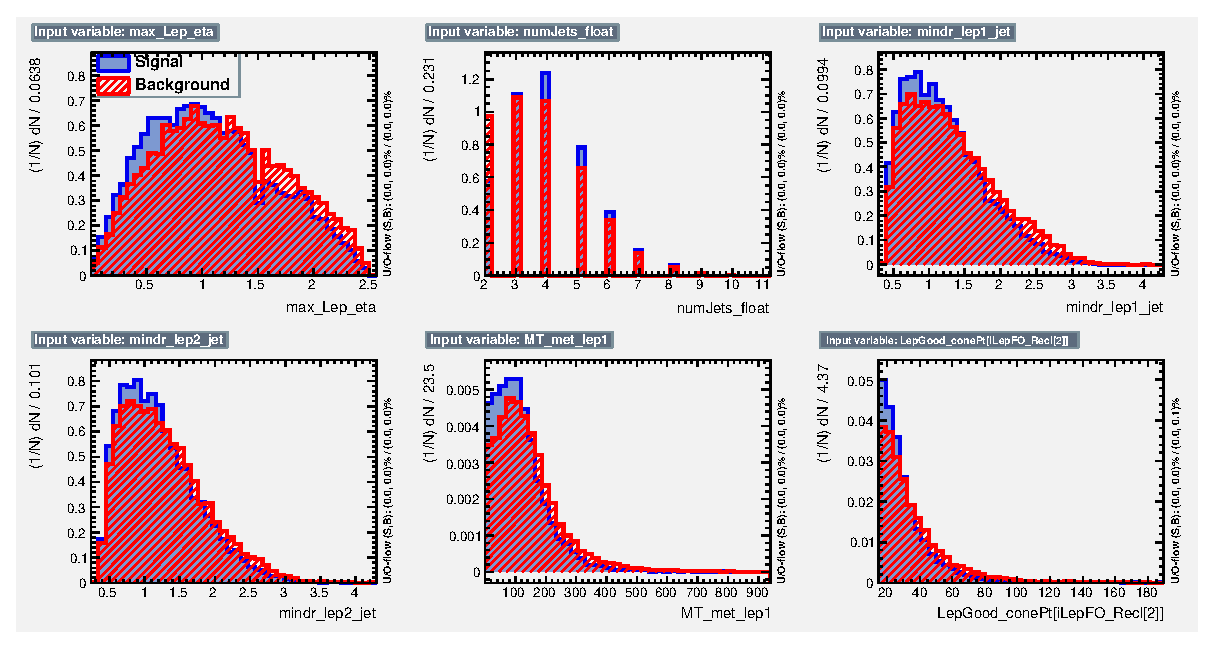
\includegraphics[width=\textwidth]{plots_extraction/training/train_3l_ttv/variables_id_c1}\\
 \includegraphics[width=\textwidth]{plots_extraction/training/train_3l_ttv/variables_id_c2}\\
\end{figure}
\begin{figure}[htb]
 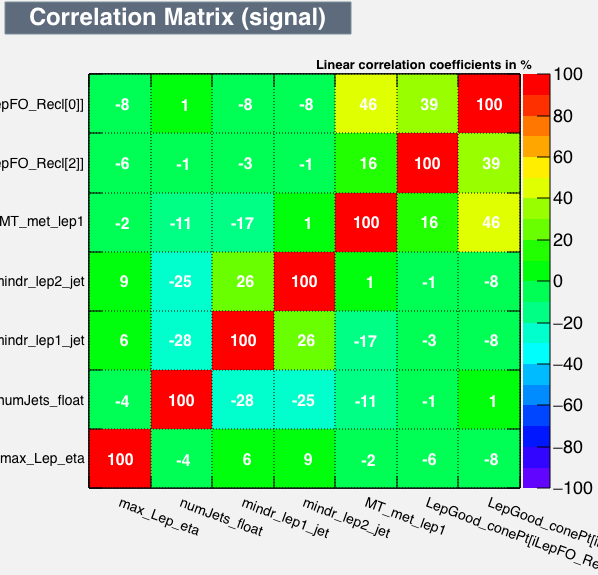
\includegraphics[width=0.32\textwidth]{plots_extraction/training/train_3l_ttv/CorrelationMatrixS}
 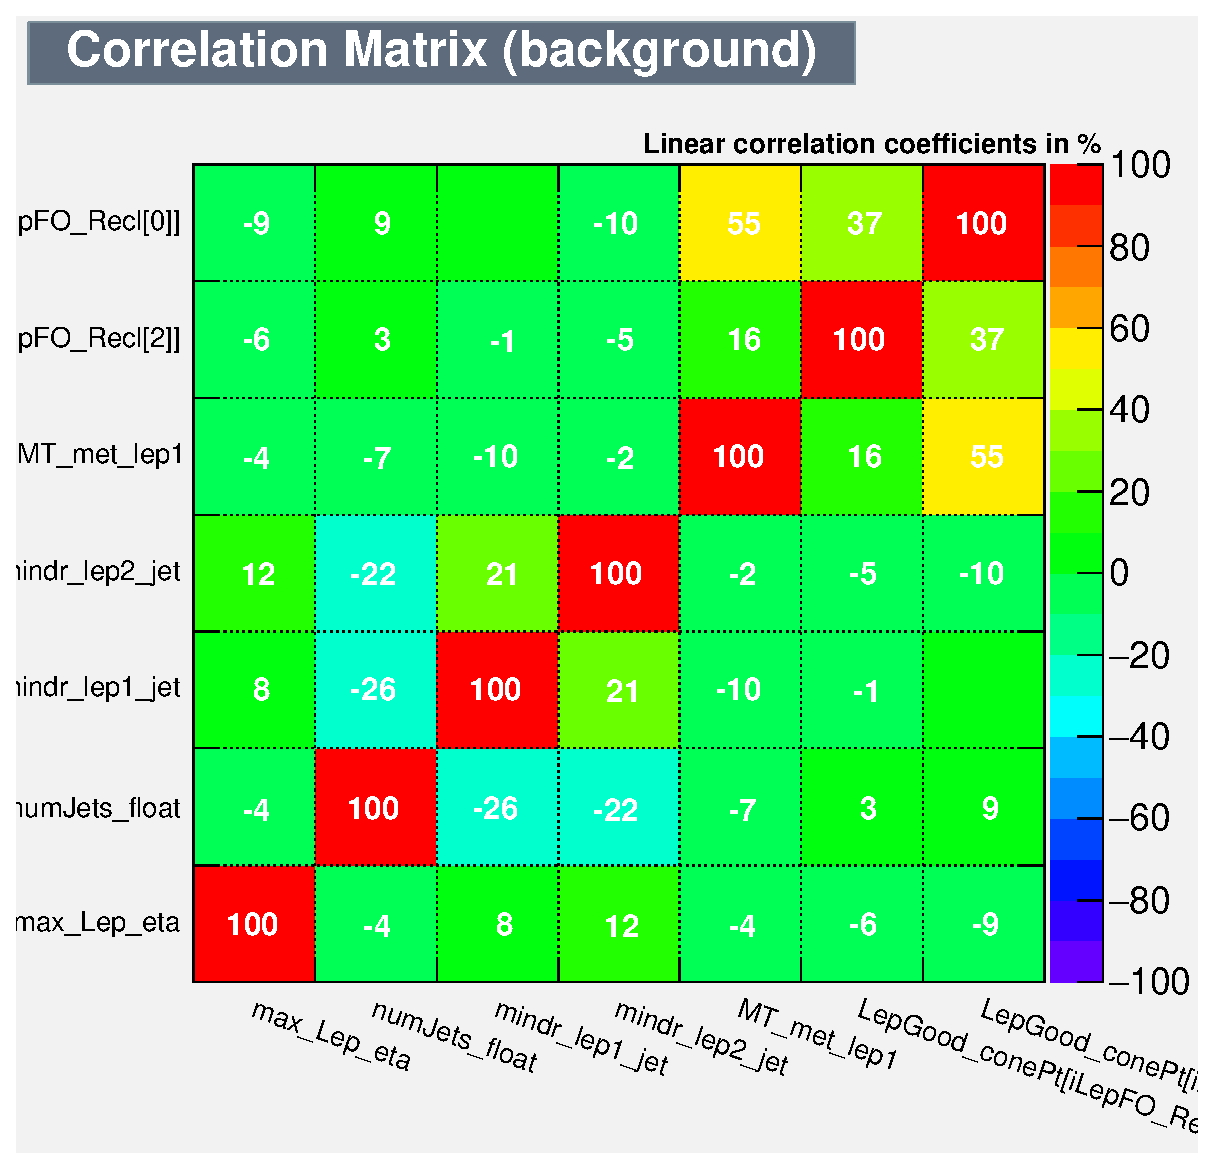
\includegraphics[width=0.32\textwidth]{plots_extraction/training/train_3l_ttv/CorrelationMatrixB}
 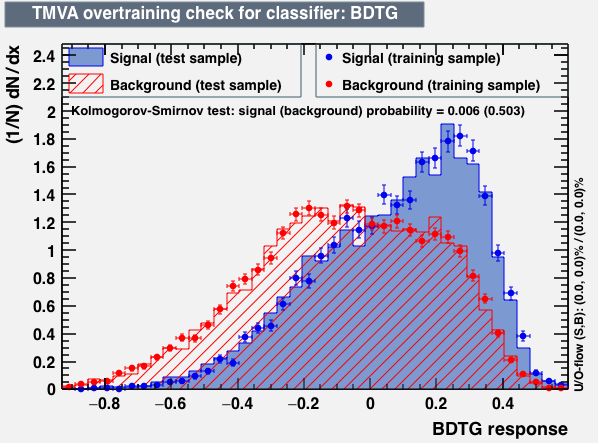
\includegraphics[width=0.32\textwidth]{plots_extraction/training/train_3l_ttv/overtrain_BDTG.png}
\end{figure}

\clearpage
